\documentclass{exam}
\usepackage{mainExam}

\title{Suites Arithmétiques : Contrôle}
\date{27 Septembre 2024}
\author{Terminale STMG 2}

\begin{document}
\maketitle
\instructions

\vspace*{1cm}
\begin{questions}
\titledquestion{Questions de cours}[3]
Soit $(u_n)$ une suite arithmétique de raison $r = 4$ et de premier terme $u_0 = 3$.

\begin{parts}
\part Comment obtient-on un terme de la suite grâce au terme précédent ?
\part Rappeler la formule explicite du terme $u_n$.
\part À quoi correspond la notation $\sum_{i = 0}^{10} u_i$ ?
\end{parts}

\vspace*{1cm}

\titledquestion{Calcul de termes}[5]
Pour chaque suite arithmétique $(u_n)_{n \in \N}$ décrite ci-après, calculer $u_7$ :
\begin{parts}
\part Le premier terme de $(u_n)_{n \in \N}$ est $u_0 = 12$ et sa raison est de $r = 8$.
\part Le premier terme de $(u_n)_{n \in \N}$ est $u_0 = 41$ et sa raison est de $r = -2$.
\part On a $u_6 = 24$ et $u_8 = 32$.
\part On a $u_2 = 10$ et $u_3 = 15$
\part On a $u_9 = 6$ et $u_{11} = 12$
\end{parts}

\vspace*{1cm}

\titledquestion{Sondage}[5]
Une campagne électorale dans un certain pays oppose deux candidats : Donald et Kamala. La côte de popularité des deux candidats est mesurée tous les premiers du mois à partir de Janvier ($n = 0$). La suite $(d_n)$ représente la côte de popularité de Donald chaque mois, tandis que la suite $(k_n)$ représente celle de Kamala. La figure ci-contre montre l'évolution de leur côte de popularité sur $12$ mois. La popularité de Donald est de $64$ en Janvier, et celle de Kamale est de $24$.

\begin{center}
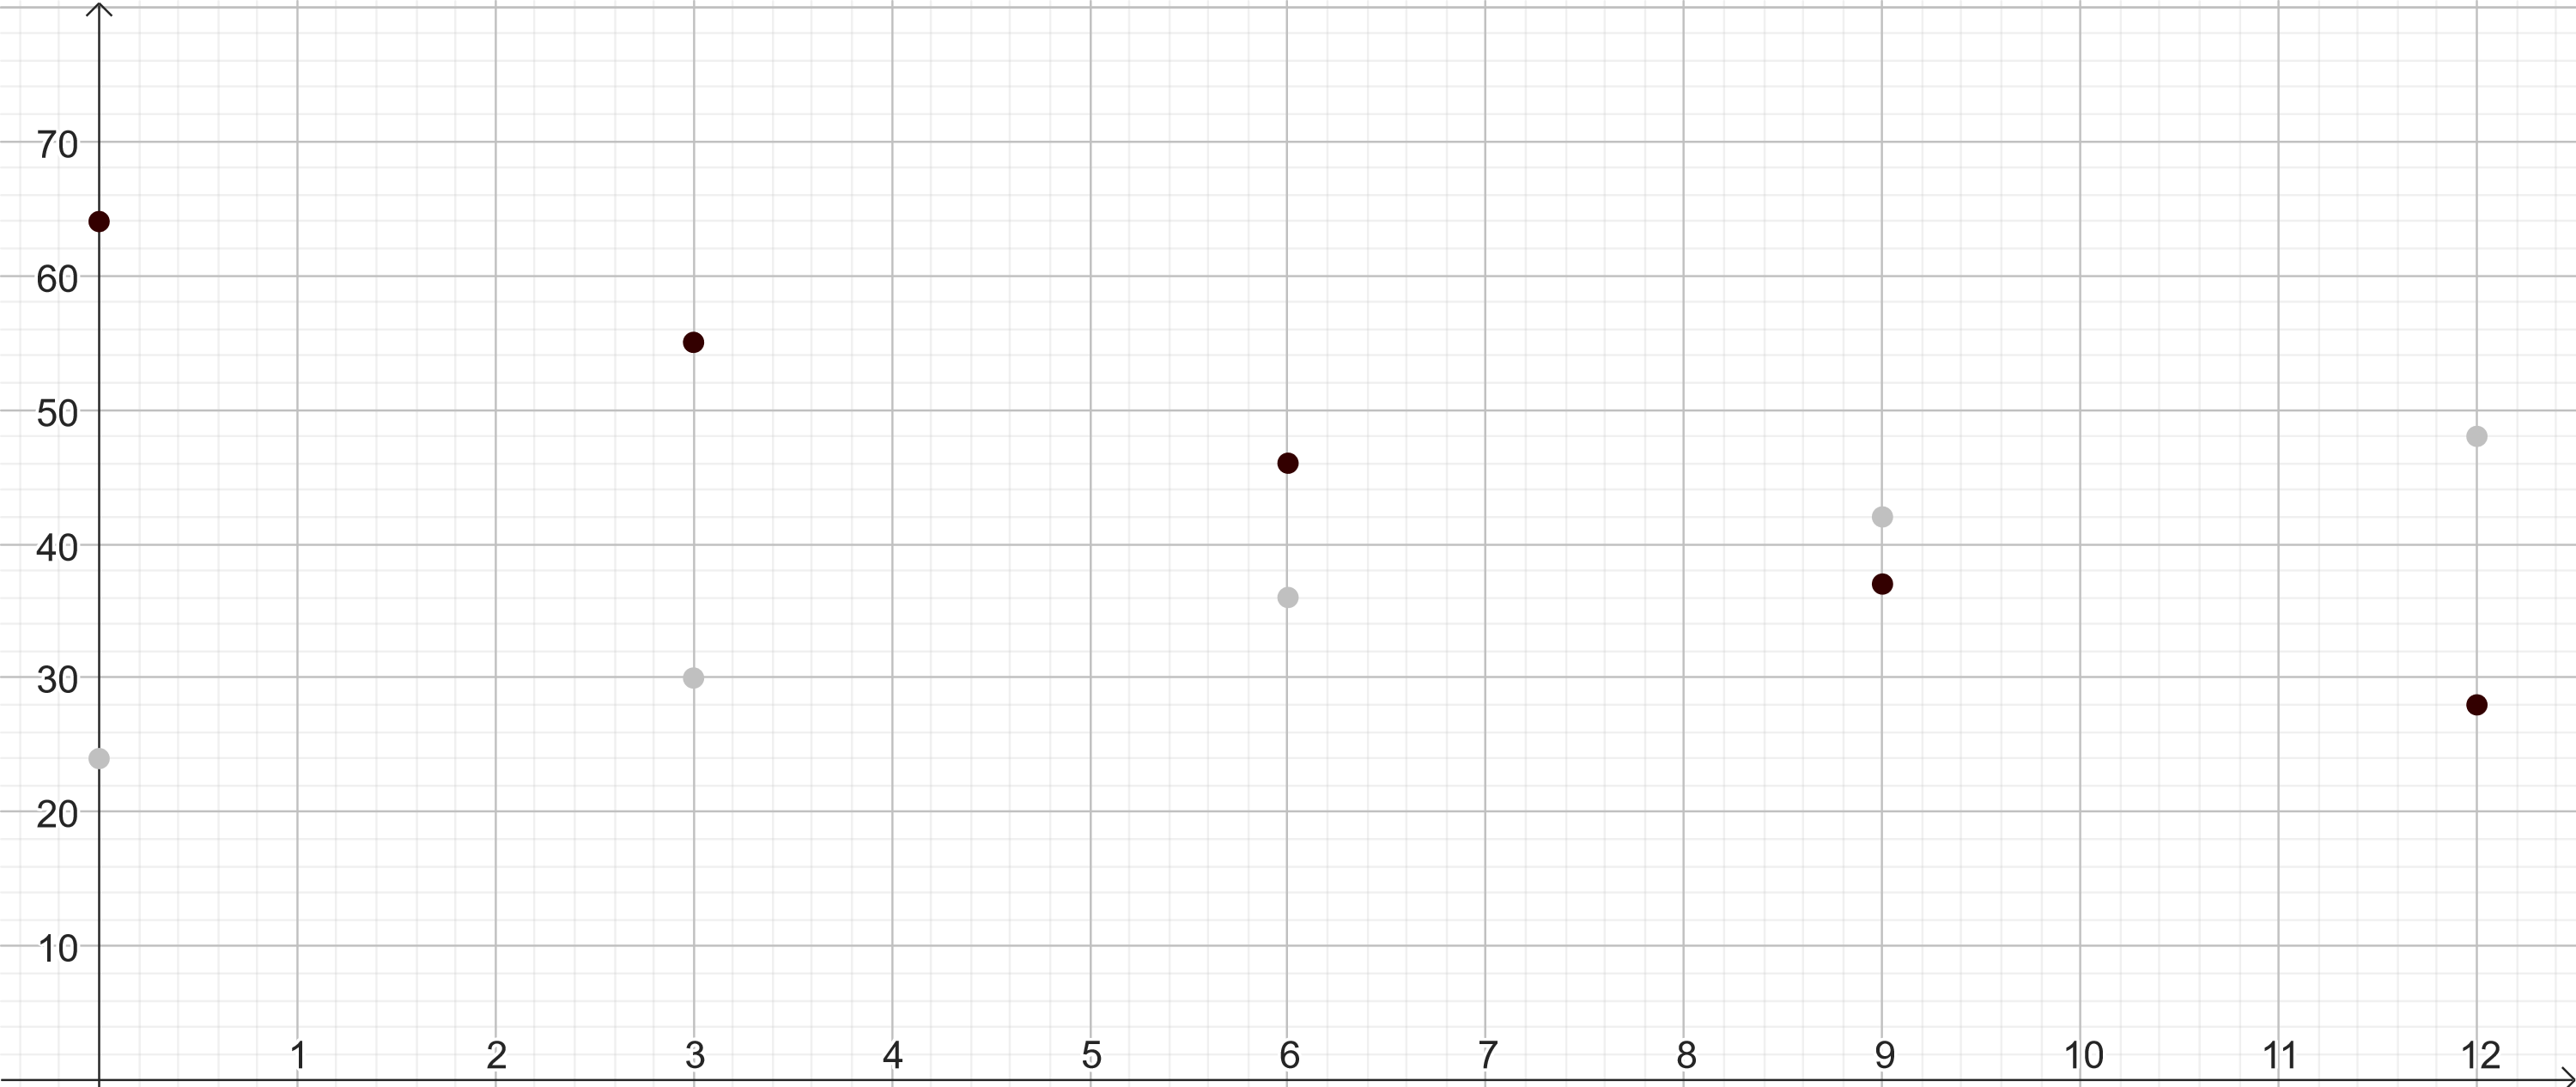
\includegraphics[width=\textwidth]{Sondage.png}
\end{center}

\begin{parts}
\part Ajouter à la figure une légende indiquant quelle série de points représente la popularité de Donald et laquelle représente celle de Kamala.
\part Justifier que les suites $(d_n)_{n \in \N}$ et $(k_n)_{n \in \N}$ sont arithmétiques, et préciser si elles sont croissantes ou décroissantes.
\part Donner la raison de ces suites.
\part À l'aide du graphique, établir le mois $n$ à partir duquel le candidat favori change.
\end{parts}

\vspace*{1cm}
\titledquestion{Marketing}[5]
Une entreprise de voyage lance une campagne marketing pour les vacances d'hiver. Le succès de la campagne est mesuré en nombre de clics sur leur site par jour. Le jour $0$, le site a enregistré $200$ clics. Contre $160$ clics au jour $1$ et $130$ au jour $2$.
\begin{parts}
\part Si on note $(c_n)_{n \in \N}$ la suite des clics au jour $n$, la suite $(c_n)$ est-elle arithmétique ?
\part Changer le nombre de clics au jour $2$ pour que la suite reste arithmétique a priori. Donner son premier terme et sa raison.
\part À l'aide de la méthode de votre choix (en résolvant une inéquation ou en traçant une représentation graphique), établir à partir de quel jour $n$ le site génère moins de $50$ clics. 
\end{parts}
\end{questions}
\end{document}